\documentclass[notheorems, handout]{beamer}

\usetheme{Warsaw}
\setbeamertemplate{page number in head/foot}[totalframenumber]
\setbeamertemplate{headline}{}
\setbeamertemplate{navigation symbols}{}
\usefonttheme[onlymath]{serif}

\usepackage[utf8]{inputenc}
\usepackage[T2A]{fontenc}
\usepackage[russian]{babel}

\usepackage{graphicx,subcaption,ragged2e}
\usepackage{tikz}
\usepackage{bm}
\usepackage{amsfonts}

\newtheorem{theorem}{Теорема}
\newtheorem{definition}{Определение}
\newtheorem{remark}{Замечание}

\title[Статистическое и машинное обучение]{Решающие деревья. Random Forest. Бустинг.}

\institute[Санкт-Петербургский Государственный Университет]{%
	\small
	Санкт-Петербургский государственный университет\\
	Кафедра статистического моделирования
}

\date[Сентябрь 2025]{Санкт-Петербург, 2025}

\begin{document}

\begin{frame}
    \titlepage
\end{frame}

\begin{frame}{Решающие деревья}
\textbf{Решающее дерево}~--- это бинарное дерево, где
\begin{itemize}
	\item во всех внутренних вершинах $v$ задан некоторый предикат $\beta_{v}: \mathbf{X} \to {0{,} 1}$,
	\item в каждой листовой вершине $v$ задан прогноз $c_{v} \in \mathbf{Y}$ (для классификации возможно: $c_{v} \in \mathbb{R_{+}^{K}}$, \; $\displaystyle\sum_{k = 1}^{K} c_{v_{k}} = 1$~--- вектор вероятностей принадлежности к классу).
\end{itemize}
\par\smallskip
\begin{figure}[h!]
  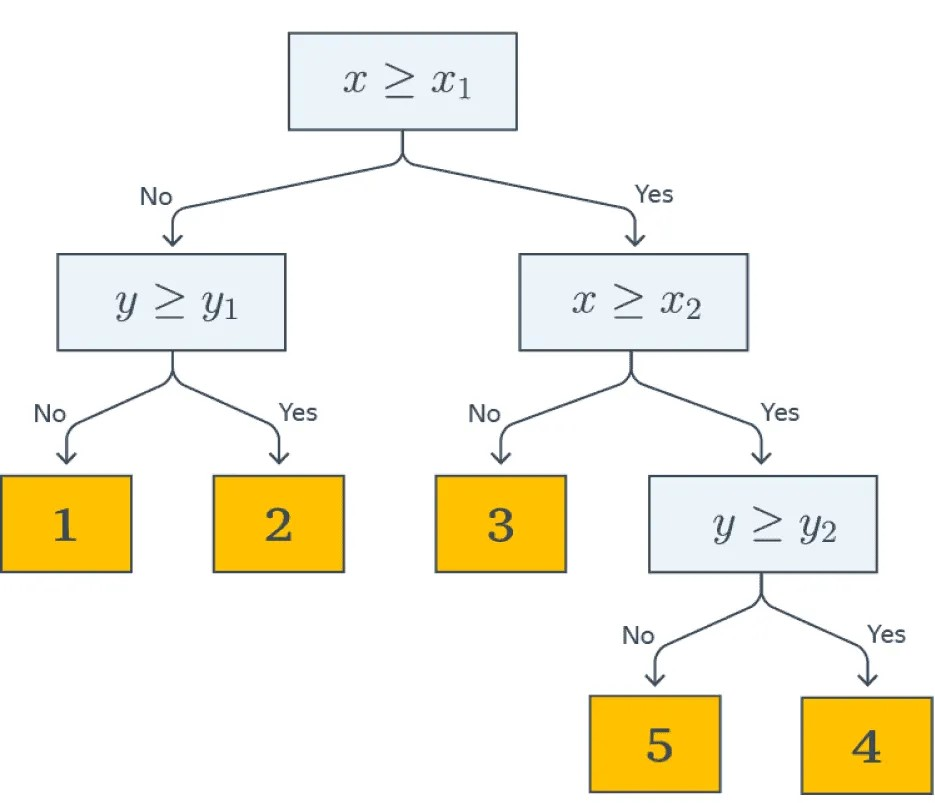
\includegraphics[width=0.4 \textwidth]{img/detree}
 \caption{Решающее бинарное дерево}
 \end{figure}
\end{frame}

\begin{frame}{Постановка задачи}
Решающие деревья можно применять как для задач регрессии,
так и для задач классификации. 
\par\smallskip
Пусть $\mathbf{X}$~--- множество объектов, $\mathbf{Y}$~--- множество ответов, $y: \mathbf{X} \to \mathbf{Y}$~--- некоторая зависимость.
\par\smallskip
Есть обучающая выборка $\mathbf{D} = \{(x_{i}{,} \; y_{i})\}_{i = 1}^{n}$, где $x_{i}$~--- входные данные, $y_{i}$~--- известные ответы.
\par\smallskip
\begin{itemize}
	\item $y_{i} \in \{1{,}\dots{,}\;K\} \Rightarrow$ задача классификации.
	\item $y_{i} \in \mathbb{R} \Rightarrow$ задача регрессии.
\end{itemize}
\end{frame}

\begin{frame}{Решающие деревья в задаче регрессии}
Пусть $\mathbf{X} \in \mathbb{R}^{n \times p}$~--- матрица данных (где $p$~--- признаки, $n$~--- наблюдения), $\mathbf{Y} \in \mathbb{R}^{n}$~--- отклик.
\par\smallskip
\textbf{Идея}: разбиение совокупности всех возможных значений  $\mathbf{X}_{1}, \dots{,}\; \mathbf{X}_{p}$ на $J$ непересекающихся областей $R_{1}, \dots{,}\; R_{J}$.
\par\smallskip
Предсказание для объекта $x$:
\begin{flalign*}
	f(x) = \displaystyle\sum_{j = 1}^{J} c_{j} \mathbf {1}(x \in R_{j}).
\end{flalign*}
Многомерные прямоугольники $R_{1}, \dots{,}\; R_{J}$ выбираем так, чтобы минимизировать сумму квадратов остатков:
\begin{flalign*}
	RSS = \displaystyle\sum_{j = 1}^{J}\displaystyle\sum_{i \in \mathbf{R}_{j}}{(y_{i} - f(x_{i}))}^{2} \rightarrow \min_{R_{1}, \dots{,}\; R_{J}}.
\end{flalign*}
Тогда
\begin{flalign*}
	\hat{c}_{j} = \frac{1}{|R_{j}|} \displaystyle\sum_{x_{i} \in R_{j}} y_{i}.
\end{flalign*}
\end{frame}

\begin{frame}{Решающие деревья в задаче регрессии}
\begin{figure}[h!]
  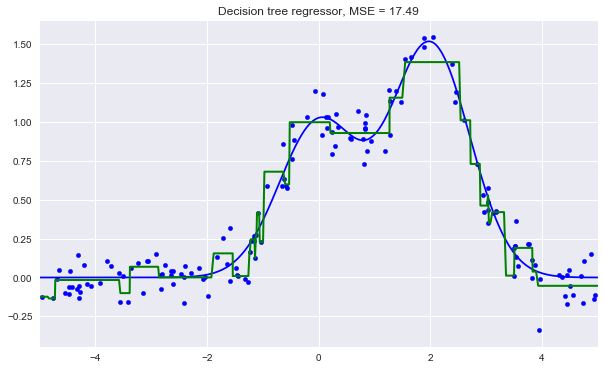
\includegraphics[width=1 \textwidth]{img/retree}
 \caption{Использование решающих деревьев в задачах регрессии}
 \end{figure}
\end{frame}

\begin{frame}{Решающие деревья в задаче классификации}
В задаче классификации $R_{1}, \dots{,}\; R_{J}$ минимизируется число ошибок классификации
\begin{flalign*}
	M(j) = 1 - \max_{k}(\hat{p}_{jk}),
\end{flalign*}
где $\hat{p}_{jk}$~--- доля объектов обучающей выборки класса $k$ попавших в $R_{j}$.
\par\smallskip
На практике чаще используют две других метрики:
\begin{itemize}
	\item $G(j) = \displaystyle\sum_{k = 1}^{K} \hat{p}_{jk} (1 - \hat{p}_{jk})$~--- индекс Джини,
	\item $CI(j) = -\displaystyle\sum_{k = 1}^{K} \hat{p}_{jk} \log{\hat{p}_{jk}}$~--- коэффициент перекрестной энтропии.
\end{itemize}
Предсказание для объекта x:
\begin{flalign*}
	f(x) = \underset{k \in \mathbf{Y}}{\operatorname{argmax}}\; \hat{p}_{jk}.
\end{flalign*}
\end{frame}

\begin{frame}{Решающие деревья в задаче классификации}
\begin{columns}
	\begin{column}{0.5\textwidth}
		\begin{figure}[h!]
		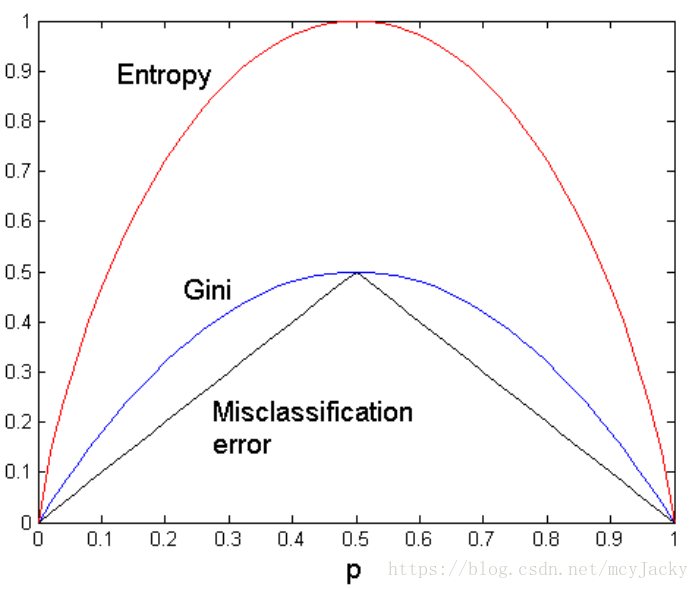
\includegraphics[width=\textwidth]{img/gini_entropy.png}
		\caption{Информационные индексы M, G, CI в случае двух классов}
		\end{figure}
	\end{column}
	\begin{column}{0.5\textwidth}
		\begin{figure}[h!]
		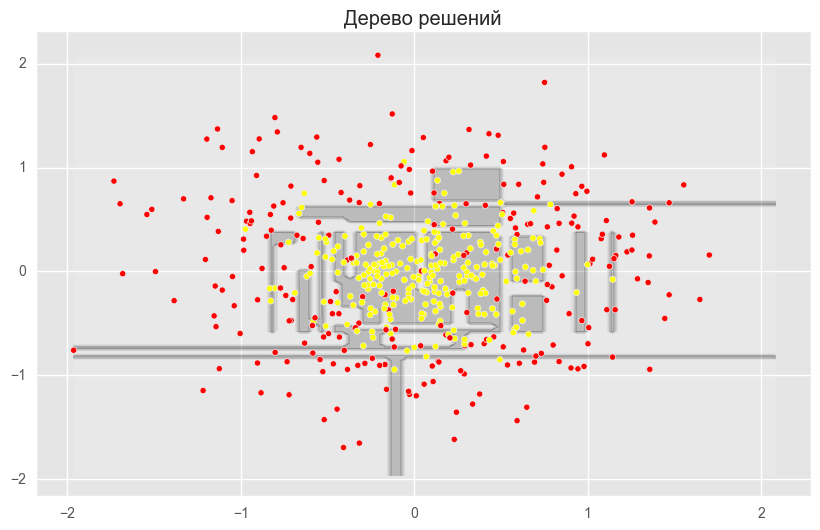
\includegraphics[width=\textwidth]{img/cltree2}
		\caption{Использование решающих деревьев в задачах классификации}
		\end{figure}
	\end{column}
\end{columns}
\end{frame}

\begin{frame}{Жадный алгоритм построения решающего дерева}
Нахождение оптимального дерева~--- это NP-полная задача.

Пусть $X$~--- исходное множество обучающей выборки, а $X _m$ — множество объектов, попавших в текущий лист (в самом начале $X _m = X$). Тогда жадный алгоритм можно верхнеуровнево описать следующим образом:

\begin{enumerate}
	\item Создаём вершину $v$;
	\item Если выполнен критерий остановки $\mathrm{Stop}(X _m)$, то останавливаемся, объявляем эту вершину листом и ставим ей в соответствие ответ $\mathrm{Ans}(X _m)$, после чего возвращаем её;
	\item Иначе: находим предикат $B _{j, t}$ (сплит), который определит наилучшее разбиение текущего множества объектов $X _m$ на две подвыборки $X _l$ и $X _r$, максимизируя критерий ветвления $\mathrm{Branch}(X _m, j, t)$;
	\item Для $X _l$ и $X _r$ рекурсивно повторим процедуру.
\end{enumerate}

% \begin{itemize}
% 	\item Выбираем признак $j$ и порог $t$ так, чтобы разбиение $\mathbf{X}^{(n)}$ на $R_{1}(j, t) = \{x \in \mathbf{X}^{(n)}| \mathbf{X}_{j} < t\}$ и $R_{2}(j, t) = \{x \in \mathbf{X}^{(n)}| \mathbf{X}_{j} \geq t\}$ решало оптимизационную задачу:
% 	\begin{flalign*}
% 		\displaystyle\sum_{i: x_{i} \in R_{1}(j, t)} {(y_{i} - \hat{y}_{R_{1}})}^{2} + \displaystyle\sum_{i: x_{i} \in R_{2}(j, t)} {(y_{i} - \hat{y}_{R_{2}})}^{2} \rightarrow \min_{j, t},
% 	\end{flalign*}
% где $\hat{y}_{R_{l}} = \frac{1}{|R_{l}|} \displaystyle\sum_{i: x_{i} \in R_{l}(j, t)} y_{i}, \;\;\; l = 1, 2$.
% 	\item Разбиваем выборку на области $R_{1}$ и $R_{2}$, образуя две дочерние вершины.
% 	\item Повторяем процедуру в пределах каждой получаемой области, пока не выполнится один из критериев останова.
% \end{itemize}
На выходе получаем дерево, в каждом из листов которого содержится по крайней мере один объект исходной выборки. 
\end{frame}

\begin{frame}{Значение листа}
$\mathrm{Ans}(X _m)$ вычисляет ответ для листа по попавшим в него объектам из обучающей выборки. Может быть:

\begin{enumerate}
	\item в случае задачи классификации — меткой самого частого класса или оценкой дискретного распределения вероятностей классов для объектов, попавших в этот лист;
	\item в случае задачи регрессии — средним, медианой или другой статистикой;
	\item простой моделью. К примеру, листы в дереве, задающем регрессию, могут быть линейными функциями или синусоидами, обученными на данных, попавших в лист.
\end{enumerate}
\end{frame}

\begin{frame}{Критерии остановки}
Критерий остановки $\mathrm{Stop}(X _m)$~--- функция, которая решает, нужно ли продолжать ветвление или пора остановиться.

\begin{itemize}
	\item Ограничение максимальной глубины дерева.
	\item Ограничение минимального числа объектов в листе.
	\item Ограничение максимального количества листьев в дереве.
	\item Остановка в случае, если все объекты в листе относятся к одному классу.
	\item Остановка в случае, если изменение метрики меньше порога.
\end{itemize}
\begin{remark}
	Для очень глубоких деревьев имеем переобучение.
\end{remark}
\end{frame}

\begin{frame}{Критерий ветвления}
	$\mathrm{Branch} (X _m, \text{feature}, \text{value})$~--- функция, измеряющая, насколько улучшится финальная метрика дерева при предлагаемом сплите.

	Пусть $L (y _i, c)$~--- функция потерь, $c$~--- константное предсказание. Информативность узла (хотим минимизировать):
	\[
	H (X _m) = \frac 1 {|X _m|} \sum _{(x _i, y _i) \in X _m} L (y _i, c).
	\]
	Если разделить на два узла:
	\[
	\begin{aligned}
		&\frac 1 {|X _m|} \left(\sum _{(x _i, y _i) \in X _l} L (y _i, c _l) + \sum _{(x _i, y _i) \in X _r} L (y _i, c)\right) =\\
		&= \frac {|X _l|} {|X _m|} H (X _l) + \frac {|X _r|} {|X _m|} H (X _r).
	\end{aligned}
	\]
\end{frame}

\begin{frame}{Критерий ветвления}
	Тогда критерий ветвления:
	\[
	\mathrm{Branch} (X _m, j, t) = |X _m| \cdot H(X _m) - |X _l| \cdot H(X _l) - |X _r| \cdot H(X _r).
	\]
	Чем больше изменение метрики, тем лучше.

	\begin{itemize}
		\item MSE: $L (y _i, c) = (y _i - c) ^2$, $H (X _m) = \sum \limits _{(x _i, y _i) \in X _m} \frac {(y _i - \overline{y}) ^2} {|X _m|}$;
		\item MAE: $L (y _i, c) = |y _i - c|$, $H (X _m) = \sum \limits _{(x _i, y _i) \in X _m} \frac {|y _i - \mathrm{MEDIAN}(Y _m)|} {|X _m|}$;
		\item Для классификации можно рассматривать: misclassification error ($H (X _m) = 1 - \max p _i$, $p _i$~--- доля класса $i$), энтропию ($H (X _m) = - \sum ^K _{k = 1} p _k log p_k$) или критерий Джини ($H (X _m) = \sum ^K _{k = 1} p _k (1 - p_k)$).
	\end{itemize}
\end{frame}

\begin{frame}{Стрижка деревьев(pruning tree)}
\begin{itemize}
	\item \textbf{Проблема}: переобучение~--- небольшое смещение, но большая дисперсия.
	\item \textbf{Решение}: объединяя некоторые $R_{j}$ можем уменьшить дисперсию за счет небольшого увеличения смещения.
	\item Выращиваем дерево только до тех пор, пока уменьшение функции потерь из-за разбиения превышает некоторый (высокий) порог.
	\item Однако можно пропустить хорошее разбиение, остановившись слишком рано. Поэтому можно выращивать большие деревья $T_{0}$, а затем обрезать его для получения поддерева.
\end{itemize}
\end{frame}

\begin{frame}{Cost-complexity pruning}
\begin{itemize}
	\item Получим большое дерево $T_{0}$ и обрежем его в узле $t$, получив поддерево $T^{t} \subset T_{0}$.
	\item Рассмотрим последовательность деревьев проиндексированных положительным параметром $\alpha$. Каждому $\alpha$ соответствует поддерево $T \subset T_{0}$, минимизирующее критерий
		\begin{flalign*}
			Q_{\alpha}(T) = Q(T) + \alpha |l(T)|,
		\end{flalign*}
где $Q(T)$~--- разница между прогнозируемым и фактическим выходом модели на этапе её обучения, $\alpha \geq 0$, $|l(T)|$~--- число листьев в поддереве $T$. 
	\item Выберем $\alpha$ с помощью кросс-валидации и возьмем соответствующее поддерево.
\end{itemize}
\end{frame}

\begin{frame}{Преимущества и недостатки решающих деревьев}
\textbf{Преимущества}:
\begin{itemize}
	\item Простота интерпретации.
	\item Пригодность и для задач регрессии, и для задач классификации.
	\item Легко визуализировать.
	\item Возможность работы с пропусками в данных.
\end{itemize}

\textbf{Недостатки}:
\begin{itemize}
	\item Метод явялется неустойчивым и склонным к переобучению.
\end{itemize}
\end{frame}

\begin{frame}{Bagging}
\textbf{Bagging} --- метод, который позволяет уменьшить разброс модели. Этот метод обучает некоторое число алгоритмов так, что каждый алгоритм обучается на отдельных выборках, которые получены из исходной посредством бутстрапа.
\par\smallskip
Разложение MSE в задаче регрессии:
\begin{flalign*}
	MSE=(\eta-\mathbf{E}\hat{\eta})^2 + \mathbf{E}(\mathbf{E}\hat{\eta} - \hat{\eta})^2
\end{flalign*}
\par\smallskip
Разброс для ансамбля с усреднением, $\hat{\eta}=\frac{1}{M}\sum_{i=1}^M\hat{\eta}_i$:
\begin{flalign*}
	\mathbf{D}[\hat{\eta}]=\frac{1}{M^2}\sum_{i=1}^M \mathbf{D}[\hat{\eta}_{i}]+\frac{1}{M^2}\sum_{i \neq j} \mathbf{cov}(\hat{\eta}_i, \hat{\eta}_j)
\end{flalign*}
\end{frame}

\begin{frame}{Ансамбли}
Набор алгоритмов называется \textbf{ансамблем}, предсказание ансамбля в бэггинге:
\begin{flalign*}
	a_{M}(x) = \frac{1}{M} \sum_{m=1}^{M} b_{m}(x)
\end{flalign*}
\par\smallskip
Смещение бэггинга совпадает со смещением базового алгоритма. При этом если базовые алгоритмы \textbf{некоррелированы}, то разброс уменьшается в $M$ раз.
\end{frame}

\begin{frame}{Random Forest}
Модель \textbf{Random Forest} --- улучшение бэггинга решающих деревьев. Деревья становятся менее коррелированными благодаря тому, что при построении дерева в каждой вершине признак выбирается из случайного подмножества заданного размера $p$. Например, $p=\sqrt{d}$, где $d$ --- число признаков, для регрессии.
\par\smallskip
Ограничения в построении дерева выбираются так, чтобы деревья получались глубокими --- такие деревья имеют низкое смещение.
\end{frame}

\begin{frame}{Gradient Boosting}
\textbf{Бустинг} --- метод ансамблирования, в котором каждый добавляемый в композицию алгоритм обучается на ошибки ансамбля на предыдущем шаге.
\par\smallskip
\textbf{Пример}: Рассмотрим задачу регрессии
\begin{flalign*}
	\frac{1}{2}\sum_{i=1}^{N}(a(x_i)-y_i)^2\rightarrow\min_{a}.
\end{flalign*}
\par\smallskip
Пусть предсказание алгоритма --- сумма предсказаний некоторых других базовых моделей:
\begin{flalign*}
	a_M(x)=\sum_{m=1}^Mb_{\theta_m, m}(x).
\end{flalign*}
\par\smallskip
Построим первый базовый алгоритм:
\begin{flalign*}
	b_{\theta_1, 1}(x)=\mathsf{argmin}_{\theta}\frac{1}{2}\sum_{i=1}^N(b_{\theta}(x_i)-y_i)^2,
\end{flalign*}
\end{frame}

\begin{frame}{Gradient Boosting}
Остатки:
\begin{flalign*}
	s_i^{(1)}=y_i-b_1(x_i).
\end{flalign*}
\par\smallskip
Следующий алгоритм:
\begin{flalign*}
	b_{\theta_2,2}(x)=\mathsf{argmin}_{\theta}\frac{1}{2}\sum_{i=1}^N(b_{\theta}(x_i)-s_i^{(1)})^2.
\end{flalign*}
\par\smallskip
И так далее. Заметим, что мы обучаемся на антиградиент:
\begin{flalign*}
	s_i^{(M)}=y_i-a_{M-1}(x_i)=-\frac{d}{dz}\frac{1}{2}(z-y_i)^2|_{z=a_{M-1}(x_i)}
\end{flalign*}
\par\smallskip
Это базовая реализация бустинга.
\end{frame}

\begin{frame}{Gradient Boosting}
Будем строить предсказание ансамбля как взвешенную сумму предсказаний базовых алгоритмов. Пусть имеется дифференцируемый функционал $L(y, z)$.
\begin{flalign*}
	a_M(x)=\sum_{m=0}^M\gamma_mb_{\theta_m, m}(x).
\end{flalign*}
\par\smallskip
Как инициализировать значения?
\begin{itemize}
	\item $b_0(x)=0$
	\item Классификация: $b_0(x) = \mathsf{argmax}_{y\in\mathbb{Y}}\displaystyle\sum_{i=1}^N[y_i=y]$
	\item Регрессия: $b_0(x) = \frac{1}{N}\sum_{i=1}^Ny_i$.
\end{itemize}
\par\smallskip
Добавление нового алгоритма в ансамбль:
\begin{flalign*}
	\sum_{i=1}^NL(y_i, a_{M-1}(x_i)+\gamma_Mb_{\theta_MM}(x_i))\rightarrow \min_{\theta_M, \gamma_M}.
\end{flalign*}
\end{frame}

\begin{frame}{Gradient Boosting}
\textbf{Идея}: предсказание следующего алгоритма должно быть противоположно производной $L(y, z)$ в точке $z=a_{M-1}(x_i)$. Тогда вектор сдвигов совпадает с антиградиентом $L$.
\par\smallskip
Таким образом, добавляя новый алгоритм, мы делаем шаг градиентного спуска.
\par\smallskip
Рассмотрим задачу регрессии:
\begin{flalign*}
	b_{\theta_M, M}(x) = \mathsf{argmin}_{\theta}\sum_{i=1}^N(b_{\theta}(x_i) - y_i)^2.
\end{flalign*}
\par\smallskip
После построения нового алгоритма, выбирается новый шаг:
\begin{flalign*}
	\gamma_M=\mathsf{argmin}_{\gamma\in\mathbb{R}}\sum_{i=1}^NL(y_i, a_{M-1}(x_i)+\gamma b_{\theta_M, M}(x_i)).
\end{flalign*}
\par\smallskip
Описанный метод называется градиентным бустингом.
\end{frame}

\begin{frame}{Gradient Boosting: Регуляризация}
\begin{itemize}
	\item Примитивные базовые алгоритмы плохо приближают антиградиент.
	\item Сложные базовые алгоритмы приведут к переобучению.
\end{itemize}
\par\smallskip
Решение этих проблем --- \textbf{сокращение шага}: вместо перехода в оптимальную точку делается укороченный шаг:
\begin{flalign*}
	a_M(x)=a_{M-1}(x)+\eta\gamma_Mb_{\theta_M, M}(x), \eta \in (0;1],
\end{flalign*}
$\eta$ --- шаг обучения.
\par\medskip
Другое решение: стохастический градиентный бустинг.
\end{frame}

\begin{frame}{Gradient Boosting: Классификация}	
Функция потерь для классификации:
\begin{flalign*}
	L(y, z)=\mathsf{ln}(1+e^{-yz}).
\end{flalign*}
\par\smallskip
Тогда построение базового алгоритма:
\begin{flalign*}
	b_{\theta_M, M}=\operatorname{argmin}_{\theta}\sum_{i=1}^N\left( b_{\theta}(x_i) - \frac{y_i}{1+e^{y_ia_{M-1}(x_i)}}\right)^2.
\end{flalign*}
\par\smallskip
Рассмотрим логистическую функцию потерь: 
\begin{flalign*}
	Q(a_M)=\sum_{i=1}^N\mathsf{ln}(1+e^{-y_ia_{M-1}(x_i)})e^{-y_i\gamma_Mb_{\theta_M, M}(x_i)}.
\end{flalign*}
\par\smallskip
Объекты с большим margin можно исключить.
\end{frame}

\begin{frame}{Gradient Boosting: Решающие деревья}
Градиентный бустинг деревьев --- один из самых сильных методов машинного обучения.
\par\smallskip
Представим предсказание решающего дерева в виде
\begin{flalign*}
	b_m(x)=\sum_{j=1}^{J_m}b_{mj}[x\in R_j],
\end{flalign*}
где $j$ --- индекс листа, $R_j$ --- область разбиения, $b_{mj}$ --- ответ в листе.
\par\smallskip
Предсказание ансамбля:
\begin{flalign*}
	a_M(x)=a_{M-1}(x)+\gamma_M\sum_{j=1}^{J_M}b_{M_j}[x\in R_j]=
\end{flalign*}
\par\smallskip
\begin{flalign*}
	a_{M-1}(x)+\sum_{j=1}^{J_M}\gamma_Mb_{M_j}[x\in R_j].
\end{flalign*}
\end{frame}	

\begin{frame}{Gradient Boosting: Решающие деревья}
Таким образом, добавление в ансамбль решающего дерева с $J_M$ листьями эквивалентно добавлению $J_M$ предикатов $x\in R_j$.
\par\smallskip
Градиентный бустинг может лишь снизить смещение базовых моделей, а разброс бустинга не меньше разброса базового алгоритма.
\par\smallskip
Поэтому в бустинге используются неглубокие решающие деревья, которые не склонны к переобучению.
\end{frame}

\begin{frame}{Gradient Boosting: Преимущества и недостатки }
Преимущества градиентного бустинга:
\begin{itemize}
	\item Точнее многих архитектур.
	\item Быстро обучается.
	\item Хорошо работает с категориальными признаками.
	\item Множество хороших реализаций: XGBoost, CatBoost, LightGBM, с поддержкой Map Reduce.
\end{itemize}
\par\smallskip
Недостатки:
\begin{itemize}
	\item Легко переобучается.
\end{itemize}
\end{frame}


\end{document}
